\documentclass[10pt]{article}
\usepackage[polish]{babel}
\usepackage[utf8]{inputenc}
\usepackage[T1]{fontenc}
\usepackage{amsmath}
\usepackage{amsfonts}
\usepackage{amssymb}
\usepackage[version=4]{mhchem}
\usepackage{stmaryrd}
\usepackage{graphicx}
\usepackage[export]{adjustbox}
\graphicspath{ {./images/} }

\title{GIMNAZJUM }

\author{}
\date{}


\begin{document}
\maketitle
\begin{enumerate}
  \item Czy można pokryć szachownicę o wymiarach \(13 \times 13\) klockami \(1 \times 4\) w taki sposób, że tylko środkowe pole nie jest zakryte?
  \item Na rysunku są trzy koła wzajemnie styczne, których środki są współliniowe. Udowodnij, że suma pól dwóch mniejszych kół jest równa polu zacienionej części największego koła tylko wtedy, gdy mniejsze koła mają jednakowe promienie.
  \item Oblicz sumę:\\
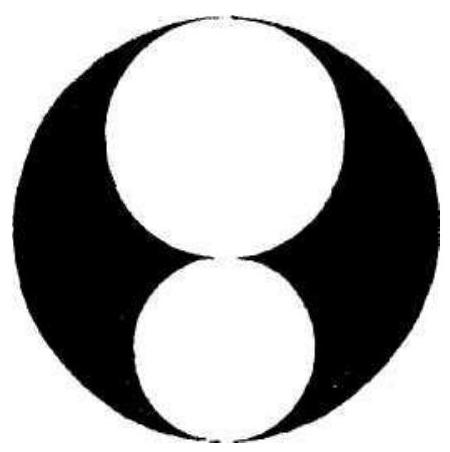
\includegraphics[max width=\textwidth, center]{2024_11_21_987c6ba970ccfad9badfg-1}
\end{enumerate}

\[
\left(2^{-2017}+1\right)^{-1}+\left(2^{-2016}+1\right)^{-1}+\cdots+\left(2^{-1}+1\right)^{-1}+\left(2^{0}+1\right)^{-1}+\left(2^{1}+1\right)^{-1}+\cdots+\left(2^{2016}+1\right)^{-1}+\left(2^{2017}+1\right)^{-1}
\]

\section*{LICEUM}
\begin{enumerate}
  \item Mamy 20 kart z liczbą 6, która staje się liczbą 9, gdy obrócimy kartę. Karty, obrócone w sposób losowy (na niektórych widzimy 6, na pozostałych 9) układamy w stos. Następnie bierzemy grupę kart, na której wierzchu jest karta z 9 i obracamy wszystkie karty. Jak ustawić karty, żeby powyższą operację można było powtarzać w nieskończoność?
  \item Udowodnij, że żaden element zbioru \(A=\{12 n+2, n \in N\}\) nie jest kwadratem liczby całkowitej.
  \item Wykaż, że (2n+2)-cyfrowa liczba \(\underbrace{11 \ldots 1}_{n} \underbrace{22 \ldots 2}_{n+1} 5\) jest, dla dowolnego n, kwadratem liczby naturalnej.
\end{enumerate}

\end{document}